\documentclass[a4paper,12pt,oneside]{book}

\usepackage[english]{babel}
\usepackage[T1]{fontenc}
\usepackage[utf8]{inputenc}

\usepackage{indentfirst,times,ragged2e}

\usepackage{hyperref}
\usepackage{enumitem}
\usepackage{setspace}
\usepackage{titlesec}
\usepackage{makecell}

\usepackage{graphicx}
\graphicspath{ {./Images/} }
\usepackage{caption}
\usepackage{subcaption}

\usepackage{verbatim}

%\usepackage{fancyhdr}
%\usepackage[top=1in,left=1.18in,right=1.3in,bottom=1in,includehead,includefoot]{geometry}

\usepackage{amsmath}
\usepackage{amssymb}
\usepackage{bm}

\usepackage{array}
\usepackage{booktabs}
\usepackage{multirow}
\usepackage{placeins}
\setlength{\heavyrulewidth}{1.5pt}
\setlength{\abovetopsep}{4pt}

\usepackage{xcolor}

\definecolor{pyforeground}{RGB}{195,198,196}
\definecolor{pybackground}{RGB}{61,67,74}
\definecolor{pykeyword}{RGB}{176,146,185}
\definecolor{pystring}{RGB}{181,188,103}
%\definecolor{pymorekw}{RGB}{134,23,153}

\usepackage{listings}
\usepackage{lstautogobble}
\usepackage{textcomp}

\lstdefinestyle{python}{
	language=Python,
	morekeywords={self, True, None},
	basicstyle=\small\ttfamily\bfseries\color{pyforeground},
	backgroundcolor=\color{pybackground},
	keywordstyle=\bfseries\color{pykeyword},
	stringstyle=\color{pystring},
	frame=single,
	upquote=true,
	tabsize=4, % tab space width
	showstringspaces=false, % don't mark spaces in strings
	autogobble=true
	%numbers=left, % display line numbers on the left
}

\definecolor{jsonbackground}{RGB}{246,246,246}
\definecolor{attributecolor}{RGB}{29,117,179}
\definecolor{valuecolor}{RGB}{179,94,20}
\definecolor{digitcolor}{RGB}{117,67,138}

% IMPORTANTE: USARE SPAZI PER INDENTARE I VALORI
\lstdefinestyle{json}{
	basicstyle=\small\ttfamily,
	backgroundcolor=\color{jsonbackground},
	string=[s]{"}{"},
	stringstyle=\color{attributecolor},
	comment=[s]{\ "}{"},
	%morecomment=[s]{[}{]},
	commentstyle=\color{valuecolor},
	literate=
	*{0}{{{\color{digitcolor}0}}}{1}
	{1}{{{\color{digitcolor}1}}}{1}
	{2}{{{\color{digitcolor}2}}}{1}
	{3}{{{\color{digitcolor}3}}}{1}
	{4}{{{\color{digitcolor}4}}}{1}
	{5}{{{\color{digitcolor}5}}}{1}
	{6}{{{\color{digitcolor}6}}}{1}
	{7}{{{\color{digitcolor}7}}}{1}
	{8}{{{\color{digitcolor}8}}}{1}
	{9}{{{\color{digitcolor}9}}}{1},
	frame=single,
	tabsize=4,
	showstringspaces=false,
	autogobble=true
}

\usepackage{xcolor}

\textwidth=400pt
% Definizione margine sinistro pagine dispari 
\oddsidemargin=20pt
% Definizione margine destro pagine pari
\evensidemargin=20pt

\begin{document}
	\begin{titlepage}
		%\newgeometry{top=1in,left=1.18in,right=1.3in,bottom=1in}
		{\large \textbf{ALMA MATER STUDIORUM - UNIVERSIT\`{A} DI BOLOGNA}}
		% Definizione linea orizzontale
		\rule[0.1cm]{14.7cm}{0.2mm}
		\\[1\baselineskip]
		\begin{center}
			\textbf{SCUOLA DI INGEGNERIA E ARCHITETTURA}\\[1\baselineskip]
			\textit{CORSO DI LAUREA MAGISTRALE IN INGEGNERIA INFORMATICA}\\[4\baselineskip]
			\textbf{PROJECT}\\[1\baselineskip]
			on\\ Computer Vision and Image Processing M\\[4\baselineskip]
			{\large \textbf{Gamma Ray Astrophysics}}\\[12\baselineskip]
			{\large Luca Bonfiglioli, Antonio Grasso}\\[6\baselineskip]
			{\large Anno Accademico 2018/2019}
		\end{center}
	\end{titlepage}

% Pagina vuota
%\newpage\null\thispagestyle{empty}\newpage

% Numerazione romana
\frontmatter 

% Indice
\tableofcontents

% Indice delle figure
%\listoffigures

% Indice delle tabelle
%\listoftables

\newpage

% Numerazione arabica
\mainmatter 

\newpage

% Interlinea 1,5
\begin{onehalfspace}

    \chapter{Problem}
    
    The main task is to analyse astronomical images taken with gamma-ray telescopes of the \textbf{Cherenkov Telescope Array (CTA)} to find gamma-ray sources into the images. 
    In particular, we need to develop a computer vision software using the \textbf{Python} programming language. This software should be able to determine whether an image contains a gamma-ray source or not. In the former case, it should also be able to locate the gamma-ray source position into the image.
    
    % TODO
    These images are in the \textbf{Flexible Image Transport System (FITS)} format, which consists of one or more Header and Data Units (HDUs), where the first HDU is called primary HDU, or primary array. In our case, the primary array contains a 2-D array of pixels, which can be seen as the 2D-histogram of the image. The FITS headers may contain image metadata. 
    
    \begin{figure}[h!]
	\centering
	\captionsetup[subfigure]{justification=centering}
	\begin{subfigure}{.3\textwidth}
		\centering
		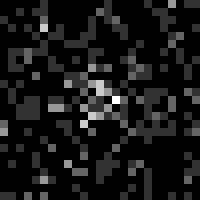
\includegraphics[width=\linewidth]{originalzoom}
		\caption{Source and background}
		\label{fig:originalzoom}
	\end{subfigure}
	\begin{subfigure}{.3\textwidth}
		\centering
		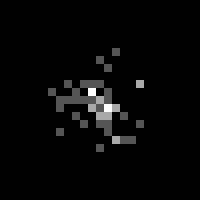
\includegraphics[width=\linewidth]{sourceonly}
		\caption{Source}
		\label{fig:sourceonly}
	\end{subfigure}
	\begin{subfigure}{.3\textwidth}
		\centering
		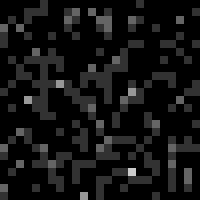
\includegraphics[width=\linewidth]{bgonlyzoom}
		\caption{Background noise}
		\label{fig:bgonlyzoom}
	\end{subfigure}
	\caption{Simulated maps showing a 25x25 pixel region}
	\end{figure}
    
    Sky maps are corrupted by noise, which may constitute an issue when trying to detect the presence and location of a gamma-ray source. \textbf{Noise} is present in two main forms:
    \begin{itemize}
		\setlength\itemsep{0em}
        \item Some photons emitted by a source are detected from a slightly different angle, this results in pixel displacement around a source, making it appear like a blob of high intensity pixels, scattered across a small region, as shown in figure \ref{fig:sourceonly};
        \item Some photons come from directions which do not correspond to any emitting source (background noise), as shown in figure \ref{fig:bgonlyzoom}.
	\end{itemize}
	The background noise is not completely uniform, but it may have some peaks and lows and if the source is weak enough it may become indistinguishable from those background noise peaks. 
	
	\chapter{Solution}
	Starting from a raw image, we observe that the region of the image corresponding to the source contains a higher density of pixels with greater intensity than the background ones. However, not all the pixels belonging to this region carry high intensity values: high intensity pixels appear scattered and mixed with low intensity ones.

	\section{Gaussian filtering}
	The first step to accomplish is denoising the raw image: this can be done by applying a \textbf{Gaussian filter}. Before applying it, we need to set $\sigma$ and the size of the kernel $s$.
	Since the interval [$-3\sigma,3\sigma$] captures $99\%$ of the area of the Gaussian function, we can assign to $s$ the closest odd integer value to $6\sigma$. We decided to bind the kernel size to a minimum of 5.
	\begin{equation}
	    s(\sigma) = \max \left( 2 \left \lfloor \frac{\left \lfloor 6\sigma \right \rfloor}{2} \right \rfloor + 1, 5 \right)
	\end{equation}
	
	We now need to choose the value of $\sigma$ in order to make it easier for us to detect the source: this depends on its shape and on the background noise in its neighbourhood. Thus, given a chosen $\sigma$, a single filtering may not be enough to detect the source, because that specific value may not be appropriate for that particular image. Therefore, we choose to apply multiple filters with increasing values of $\sigma$. \\
	Starting from an image $A$ filtered with $\sigma_{a}$ we want to obtain an image $B$ filtered with $\sigma_{b}$: if $\sigma_{b} > \sigma_{a}$, this can be easily done by filtering $A$ with $\sigma_{c} = \sqrt{\sigma_{b}^2 - \sigma_{a}^2}$. According to this formula, $\sigma_{c} < \sigma_{b}$ this means that $s(\sigma_{c}) < s(\sigma_{b})$, so filtering with $\sigma_{c}$ is less computationally expensive than filtering with $\sigma_{b}$. \\ 
    Once chosen a range of $n$ values $[\sigma_{1}, ..., \sigma_{n}]$, we can avoid filtering the original image $n$ times with $\sigma_{i}$, $i = 1, ..., n$, by instead applying $n$ consecutive filters with $\tilde{\sigma_{i}}$, $i = 1, ..., n$ where:
    
    \begin{equation}
	\tilde{\sigma}_{i} =
	    \begin{cases}
	        \sigma_{1} &\text{$i = 1$} \\ 
    	    \sqrt{\sigma_{i}^2 - \sigma_{i-1}^2} &\text{$i > 1$}
	    \end{cases}
	\end{equation}
	
	By increasing $\sigma$, as shown in figure \ref{fig:smoothed}, the source becomes more compact, its shape more circular and the pixel with the highest intensity tends to be around the center of this region.
	
	\begin{figure}
	\centering
	\captionsetup[subfigure]{justification=centering}
	\begin{subfigure}{.3\textwidth}
		\centering
		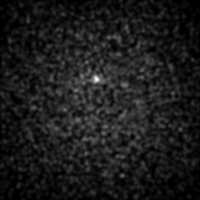
\includegraphics[width=\linewidth]{smooth3}
		\caption{Image smoothed with $\sigma=1.5$}
		\label{fig:smooth3}
	\end{subfigure}
	\begin{subfigure}{.3\textwidth}
		\centering
		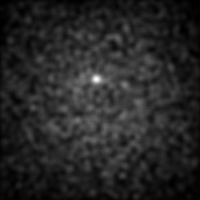
\includegraphics[width=\linewidth]{smooth5}
		\caption{Image smoothed with $\sigma=2.5$}
		\label{fig:smooth5}
	\end{subfigure}
	\begin{subfigure}{.3\textwidth}
		\centering
		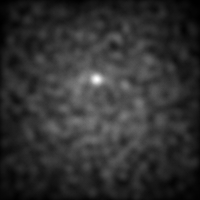
\includegraphics[width=\linewidth]{smooth7}
		\caption{Image smoothed with $\sigma=3.5$}
		\label{fig:smooth7}
	\end{subfigure}
	\caption{Image smoothed with different values of $\sigma$}
	\label{fig:smoothed}
	\end{figure} 
	
	\section{Local maxima extraction}
	If the source is present, for each filtered image we observe that there exists a local maximum which is a good approximation of the source location: the lower the $\sigma$, the better the approximation. \\
	Thus, we need to extract local maxima from each image: to do so, we iterate on each pixel checking whether it is greater than all its neighbouring pixels or not. \newpage The maxima are then stored into a list as tuples $\langle \langle x,y \rangle, i \rangle$ where $\langle x, y \rangle$ are the maxima coordinates and $i$ is their intensity. \\
	They are then sorted by decreasing values of intensity, because we know that if the source is present the corresponding local maximum will be among the most intense ones. \\
	By increasing $\sigma$ from $\sigma_i$ to $\sigma_{i+1}$ at each step, we expect some maxima found at the step $i+1$ to remain within a small range from their position at step $i$. We want these corresponding maxima to be considered as a single maximum throughout all the iterations.
	
	\section{Useful data structures}
	For this purpose, we now introduce two simple data structures: PointData and PointDataList.
	\subsection{Pointdata}
	    \setlength\itemsep{0em}
	    It lets us store values related to a specific point in the image. \\
    	\textbf{Attributes}: 
    	\begin{itemize}
    	    \setlength\itemsep{0em}
        	\item \textit{original}: a pair of coordinates initialised to a given tuple;
        	\item \textit{latest}: another pair of coordinates, initially equal to \textit{original};
        	\item \textit{r}: a numeric value initialised to a given positive value;
        	\item \textit{values}: a list of numeric values, initially empty.
    	\end{itemize}
    	\textbf{Methods}:
    	\begin{itemize}
    	\item \textit{set(c, v, i)}: it takes as input a pair of coordinates \textit{c}, a value \textit{v} and an index \textit{i}, setting \textit{latest} to \textit{c} and the i-th element of \textit{values} to the maximum value between \textit{c} and the previously stored value.
    	\item \textit{compatible(c)}: it takes as input a pair of coordinates \textit{c} and it returns a Boolean value that is true if the
    	Euclidean distance between \textit{c} and \textit{latest} is less than \textit{r}.
    	\end{itemize}
    	
    	\newpage
    	\subsubsection{Example}
    	We initialise PointData with coordinates (100, 100) and $r=5$: 
    
    	\begin{table}[!h]
            \centering
            %\caption{Comparison of percentages.}
            \begin{tabular}{*8c}
            \toprule
           \textbf{original} & \textbf{latest} & \textbf{r} & \textbf{values}\\
            \midrule
            (100, 100) & (100, 100) & 5 & $\varnothing$ \\
            \bottomrule
            \end{tabular}
        \end{table} 
    	
    	We perform the set operation with the coordinates \textbf{(101, 100)}, the value \textbf{30} and the index \textbf{0}:
    	\begin{table}[!htbp]
            \centering
            %\caption{Comparison of percentages.}
            \begin{tabular}{*8c}
            \toprule
           \textbf{original} & \textbf{latest} & \textbf{r} & \textbf{values}\\
            \midrule
            (100, 100) & \textbf{(101, 100)} & 5 & \textbf{30} \\
            \bottomrule
            \end{tabular}
        \end{table} \\ 
    	We perform another set operation with the coordinates \textbf{(101, 102)}, the value \textbf{15} and the index \textbf{4}:
    	\begin{table}[!htbp]
            \centering
            %\caption{Comparison of percentages.}
            \begin{tabular}{*8c}
            \toprule
           \textbf{original} & \textbf{latest} & \textbf{r} &  \multicolumn{5}{c}{\textbf{values}}\\
            \midrule
            (100, 100) & \textbf{(101, 102)} & 5 & 30 & 0 & 0 & 0 & \textbf{15} \\
            \bottomrule
            \end{tabular}
        \end{table} \\
    	The parameters \textit{original} and \textit{r} are intended to be read-only.
    \subsection{PointDataList}
    	It is a collection of PointData. \\
    	\textbf{Attributes}:
    	\begin{itemize}
    	    \setlength\itemsep{0em}
    	    \item \textit{points}: a list of PointData, initially empty;
        	\item \textit{r}: a numeric value initialised to a given positive value.
    	\end{itemize}
    	\textbf{Methods}:
    	    \begin{itemize}
    	    \setlength\itemsep{0em}
        	\item \textit{set(c, v, i)}: it takes as input the same parameters \textit{c}, \textit{v}, \textit{i} as those of the set operation of PointData. This	operation checks whether there is at least one element of points compatible with the coordinates \textit{c} or not:
        	in the former case it performs the set operation with the parameters \textit{c}, \textit{v}, \textit{i} on the closest compatible
        	PointData; in the latter it adds a new PointData to points and it performs the set operation on it.
        	\item \textit{get\_point(c)}: it takes as input a pair of coordinates \textit{c} returning the closest compatible element of points if any is present, nothing otherwise.
        	\end{itemize}
    	\subsubsection{Example}
    	Here we have a PointDataList already initialised with 2 PointData and some values:
    	\begin{table}[!htbp]
            \centering
            %\caption{Comparison of percentages.}
            \begin{tabular}{*8c}
            \toprule
           \textbf{original} & \textbf{latest} & \textbf{r} &  \multicolumn{5}{c}{\textbf{values}}\\
            \midrule
            (100, 100) & (101, 102) & 5 & 30 & 0 & 0 & 0 & 15\\
            (120, 100) & (121, 99) & 5  & 0  & 2 & 15 & 20 & 0\\
            \bottomrule
            \end{tabular}
        \end{table} \\
    	We perform the set operation with the coordinates \textbf{(50, 80)}, the value \textbf{18} and the index \textbf{3}. Since there is not any PointData compatible with (50, 80), a new one will be created and added to the structure:
    	\begin{table}[!htbp]
            \centering
            %\caption{Comparison of percentages.}
            \begin{tabular}{*8c}
            \toprule
           \textbf{original} & \textbf{latest} & \textbf{r} &  \multicolumn{5}{c}{\textbf{values}}\\
            \midrule
            (100, 100) & (101, 102) & 5 & 30 & 0 & 0 & 0 & 15\\
            (120, 100) & (121, 99) & 5  & 0  & 2 & 15 & 20 & 0\\
            \textbf{(50, 80)} & \textbf{(50, 80)} & \textbf{5} & \textbf{0} & \textbf{0} & \textbf{0} & \textbf{18} & \textbf{0}\\
            \bottomrule
            \end{tabular}
        \end{table} \\
    	We perform the set operation with the coordinates \textbf{(100, 101)}, the value \textbf{30} and the index \textbf{5}. (100, 101) is compatible with (101, 102), so it will perform the set operation on the first PointData:
    	\begin{table}[!htbp]
            \centering
            %\caption{Comparison of percentages.}
            \begin{tabular}{*9c}
            \toprule
           \textbf{original} & \textbf{latest} & \textbf{r} &  \multicolumn{6}{c}{\textbf{values}}\\
            \midrule
            (100, 100) & \textbf{(100, 101)} & 5 & 30 & 0 & 0 & 0 & 15 & \textbf{30}\\
            (120, 100) & (121, 99) & 5  & 0  & 2 & 15 & 20 & 0 & 0\\
            (50, 80) & (50, 80) & 5 & 0 & 0 & 0 & 18 & 0 & 0\\
            \bottomrule
            \end{tabular}
        \end{table} 
        
	\section{Features}
	For each filtered image we want now to compute a set of features for some of the maxima and store the computed values inside different PointDataList structures, one for each feature. \\
	Every feature is associated with the method \textit{update\_feature(maxima, i, point\_data\_list)}, where \textit{feature} corresponds to the feature name: it takes
	as input the sorted list of the maxima \textit{maxima}, the index \textit{i} corresponding to the i-th consecutive filtering of the image and the PointDataList \textit{point\_data\_list} to update with the computed values.
	All the features must provide higher values for maxima which are more likely to correspond to the source	and vice versa. \\s
	We have thought of two main features so far:
	\begin{itemize}
	    \setlength\itemsep{0em}
	    \item \textbf{intensity}: the intensity of the maximum under consideration. This feature is very significative and carries a lot of information about the presence of the source.
	    \item \textbf{isolatedness}: the sum of the distances between a maximum and the k nearest ones. Generally speaking, the source tends to be more isolated than the rest of the maxima, but the information provided by this feature is often useless.
	\end{itemize}
	
	\newpage
	
    We now show two graphs computed on a sky map image. In each graph, each line represents the maxima trend for a specific measure across the sigma range:
    %\FloatBarrier
	\begin{figure}[h!]
		\centering
		\captionsetup{justification=centering}
		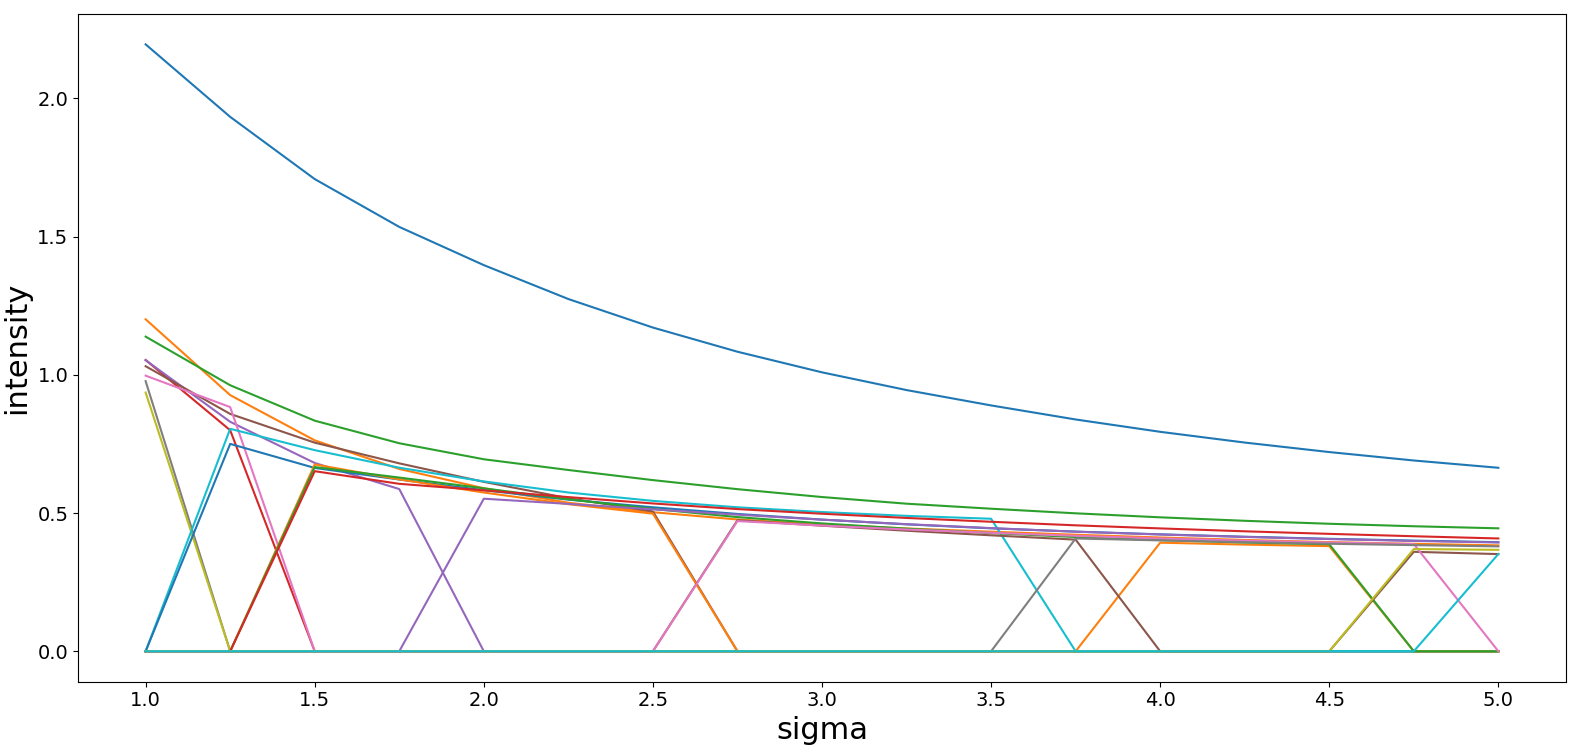
\includegraphics[width=\textwidth]{intensity}
		\caption{\textbf{Intensity} graph: we can notice a blue line significantly higher than all the others, corresponding to the source}
		\label{fig:intensity}
	\end{figure}
	
	\begin{figure}[h!]
		\centering
		\captionsetup{justification=centering}
		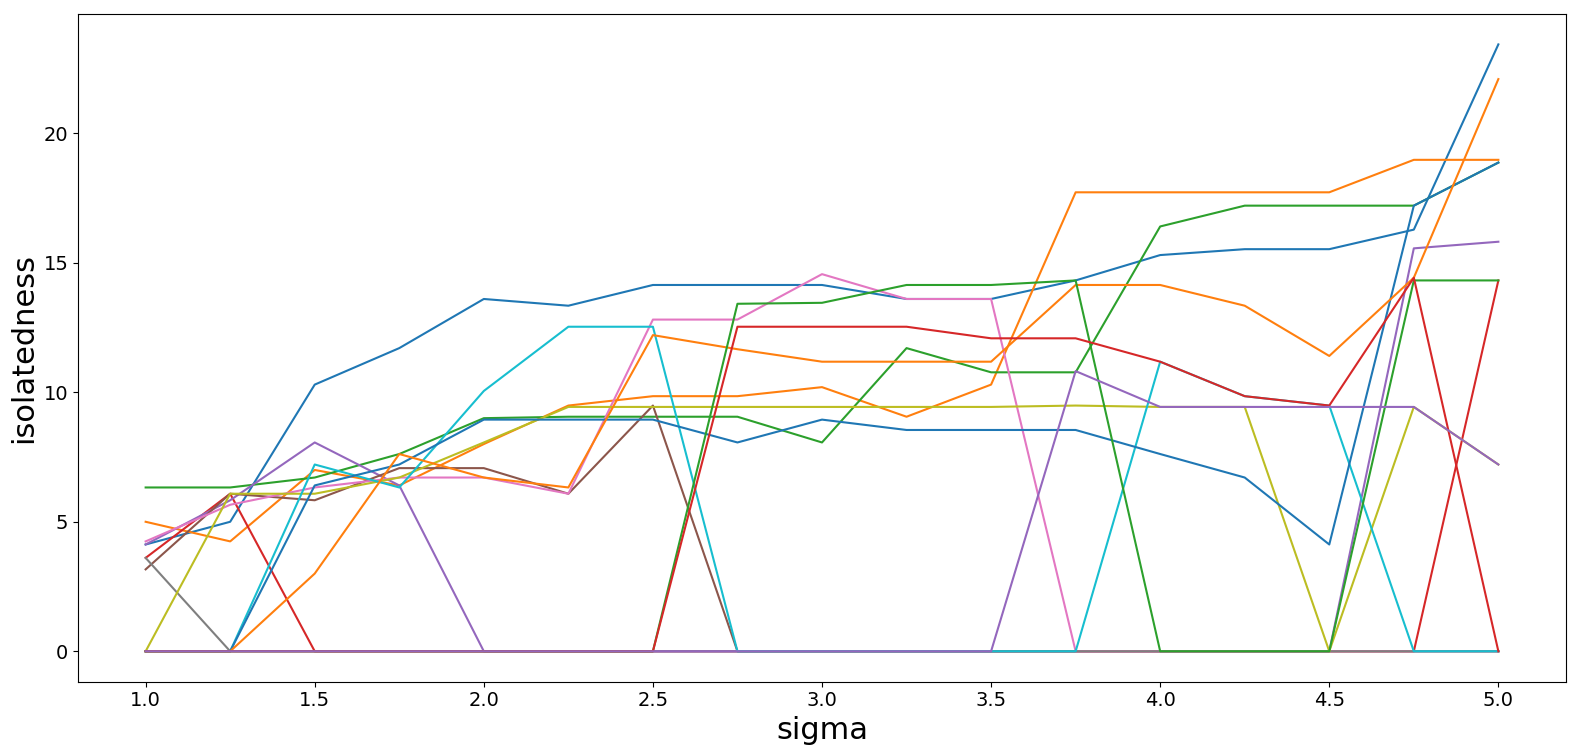
\includegraphics[width=\textwidth]{isolatedness}
		\caption{\textbf{Isolatedness} graph: we can notice a blue line significantly higher than all the others in the sigma range [1.5, 2.5], corresponding to the source}
		\label{fig:isolatedness}
	\end{figure}
	%\FloatBarrier
    
	\section{Election algorithm} \label{election_algorithm}
	After computing all the features described above for each maximum, we end up with a fully populated PointDataList for every feature (i.e. intensity, isolatedness).
	We now proceed with an election algorithm to find if there is a point which is more likely than the others to	correspond to the source, among all the points belonging to the union of all the PointDataList. For every feature and for every step ($i=1, ..., n$), we consider the two highest values $v_1$, $v_2$ ($v_1 \geq v_2$) for that particular step:
	\begin{itemize}
	    \setlength\itemsep{0em}
    	\item if $v_1 > kv_2$, $v_1$ gets $w$ votes, where $k$ and $w$ are two positive constants depending on the feature;
    	\item otherwise, the same number of votes $w$ is assigned to a special candidate that represents the absence of the source.
	\end{itemize}
	There are two possible outcomes:
	\begin{enumerate}[itemsep=0em]
    	\item The best scoring candidate is associated with a pair of coordinates which corresponds to the source;
    	\item The best scoring candidate is the one representing the absence of the source, meaning that there is no source in the image.
	\end{enumerate}
	
	\section{Configuration file}
	Along with the code, we provide a configuration file to set the most relevant parameters of the whole algorithm described so far.
	The configuration file is a JSON file that contains the following main parameters:
	\begin{itemize}
    	\setlength\itemsep{0em}
    	\item \textbf{dir}: a string representing the path containing the skymap files that the algorithm should analyse;
    	\item \textbf{sigma\_array}: a list of values [$\sigma_1$, … , $\sigma_n$] corresponding to the $\sigma_i$, $i = 1,...,n$ values needed for filtering the images;
    	\item \textbf{active\_measures}: a list of strings representing the features that the algorithm takes into account. Each feature is also associated to a parameter corresponding to the name feature (e.g. intensity, isolatedness). \\ Each of these parameters contains the lists of specific parameters needed for that particular
    	feature. Among these specific parameters there always must be four compulsory ones:
    	\begin{itemize}
        	\setlength\itemsep{0em}
        	\item \textbf{vote\_thresh}: the value of $k$ in the section “Election algorithm”
        	\item \textbf{vote\_weigth}: the value of $w$ in the section “Election algorithm”
        	\item \textbf{dist\_thresh}: the value of $r$ for the PointDataList corresponding to this feature
        	\item \textbf{method}: the name of the method that computes the feature, that method will be called automatically if the parameter \textbf{active\_measures} contains the name of this feature.
    	\end{itemize}
    \end{itemize}
	
	\chapter{Tests and Results}
	
	\section{ctools}
	We tested our algorithm on sky maps simulated using \textbf{ctools}, a software package developed for the scientific analysis of Cherenkov Telescope Array (CTA) data (\cite{tre_zero}). \\
	Before generating a sky map, we must generate an \textbf{event list} including photon events from astrophysical sources and background events from an instrumental background model (\cite{tre_uno}). To do so, we must use the \textbf{ctobssim} tool, providing the following inputs: 
	\begin{itemize}
	    \setlength\itemsep{0em}
	    \item the Right Ascension of CTA pointing $\bm{ra}$ and the Declination of CTA pointing $\bm{dec}$, in degrees;
	    \item the radius of the simulation region $\bm{rad}$, in degrees;
	    \item a time interval defined by $\bm{tmin}$ and $\bm{tmax}$, in UTC format;
	    \item an energy interval definedy by $\bm{emin}$ and $\bm{emax}$, in TeV;
	    \item an instrumental response function $\bm{irf}$;
	    \item an input XML model $\bm{inmodel}$: this is a source and background model definition file. We can set both the Right Ascension and the Declination of the source together with its flow and we can also set the background model.
	\end{itemize}
	In addition, if we want to generate different event samples in subsequent executions, we can provide a different $\bm{seed}$ for each execution.
	
	Once we have generated the event list, we can proceed generating the sky map using the \textbf{ctskymap} tool, providing the following inputs:
	\begin{itemize}
	    \setlength\itemsep{0em}
	    \item an input event list $\bm{inobs}$;
	    \item the Right Ascension of the image centre $\bm{xref}$ and the Declination of the image centre $\bm{yref}$, in degrees;
	    \item the projection method $\bm{proj}$ and the coordinate system $\bm{coordsys}$;
	    \item the pixel size $\bm{binsz}$, the size of the Right Ascension axis $\bm{nxpix}$ and the size of the Declination axis $\bm{nypix}$, in degrees;
	    \item the energy interval defined by $\bm{emin}$ and $\bm{emax}$ within events are considered, in TeV.
	 \end{itemize}
	
	\section{Sky maps generation}
	We leveraged on the ctools library to implement two main functions for the automatic sky maps generation:
	\begin{itemize}
	    \setlength\itemsep{0em}
    	\item \textbf{generate\_src\_data(start\_model, flow, n, start\_coords, radius, start\_seed)}: it generates sky maps with one source, according to the following parameters:
    	\begin{itemize}
    	    \setlength\itemsep{0em}
        	\item \textbf{start\_model}: source and background model XML file;
        	\item \textbf{flow}: flow value used for the simulations;
        	\item \textbf{n}: number of sky maps to generate;
        	\item \textbf{start\_coords}: the coordinates the source will be placed around;
        	\item \textbf{radius}: the maximum distance between start\_coords and the source;
        	\item \textbf{start\_seed}: a positive integer used as a seed for the simulation.
    	\end{itemize}
		\item \textbf{generate\_bkg\_only\_data(bkg\_only\_data, n, start\_seed)}: it generates sky maps with only the background,
        according to the following parameters:
        \begin{itemize}
            \setlength\itemsep{0em}
        	\item \textbf{bkg\_only\_model}: background model XML file;
            \item \textbf{n}: number of sky maps to generate;
        	\item \textbf{start\_seed}: a positive integer used as a seed for the simulation.
    	\end{itemize}
	\end{itemize}
	
	We generated two different sets of sky maps using the two previous methods:
	\begin{enumerate}[itemsep=0em]
	    \item The first set of \textbf{1000} sky maps was generated starting from an XML model of \textbf{both the source and the background};
	    \item The second set of \textbf{1000} sky maps was generated starting from an XML model of \textbf{only the background}, with the purpose to simulate those images which do not contain any gamma-ray source.
	\end{enumerate}
	As for the former case, we generated 1000 XML models with \textbf{source flow} equal to \textbf{2} and \textbf{source position} randomly set \textbf{within 1° from} the position \textbf{(221, 46)}. \\
	As for the latter case, we simply used the same XML model, with the only definition of the background model. \\
	The \textit{XML models} were the only variable input parameter of \textbf{ctobssim} in the event list generation process together with the $\bm{seed}$, different for every execution. The other parameters were set according to the following scheme:
	\begin{itemize}
	    \setlength\itemsep{0em}
	    \item $\bm{ra}=221$ and $\bm{dec}=46$;
	    \item $\bm{rad}=5$;
	    \item $\bm{tmin}=$ 2020-01-01T00:00:00 and $\bm{tmin}=$ 2020-01-01T00:15:00;
	    \item $\bm{emin}=0.1$ and $\bm{emax}=100$.
	\end{itemize}
    Sky maps were then generated using the following parameters for \textbf{ctskymap}:
    \begin{itemize}
	    \setlength\itemsep{0em}
	    \item $\bm{xref}=221$ and $\bm{yref}=46$;
	    \item $\bm{binsz}=0.02$;
	    \item $\bm{nxpix}=200$ and $\bm{nypix}=200$;
	    \item $\bm{emin}=0.1$ and $\bm{emax}=100$.
	\end{itemize}
	
	\newpage 
	
	\section{Results}
	After generating the two sets of sky maps previously mentioned, we tested the algorithm over them. Different executions were needed to tune the configuration file parameters in order to \textbf{minimize} both the number of background only sky maps the algorithm found a gamma-ray source in (\textbf{false positives}) and the number of source and background sky maps the algorithm did not found the gamma-ray source in (\textbf{false negatives}).
	Here is the resulting confusion matrix:
	%\FloatBarrier
	\begin{table}[h!]
        \centering
    	\begin{tabular}{l|l|c|c|c}
        \multicolumn{2}{c}{} & \multicolumn{2}{c}{Prediction} \\
        \cline{3-4}
        \multicolumn{2}{c|}{} & Positive & Negative & \multicolumn{1}{c}{Total} \\
        \cline{2-4}
        \multirow{2}{*}{\shortstack{Label}} & Positive & 997 & 3 & 1000 \\
        \cline{2-4}
        & Negative & 3 & 997 & 1000 \\
        \cline{2-4}
        \multicolumn{1}{c}{} & \multicolumn{1}{c}{Total} & \multicolumn{1}{c}{1000} & \multicolumn{1}{c}{1000} & \multicolumn{1}{c}{2000}\\
        \end{tabular}
        \caption{Confusion matrix}
    \end{table} \\
    %\FloatBarrier
	We can observe that both the \textbf{false positives rate} and the \textbf{false negatives rate} are equal to $0.3\%$.
	
	\section{Conclusions}
	Although we achieved a low error on both the false positives and the false negatives, from the purely scientific point of view we should prioritize the minimization of false positives rather than false negatives. Further parameters tuning and local analysis may be deployed to achieve better results. \\
	Another problem concerns the election algorithm mentioned in the section \ref{election_algorithm}: in order to make the algorithm work properly, $v_1/v_2$ should be scale-invariant for all the features. As for the intensity values, their ratios are clearly not scale-invariant, since values tend asymptotically to the
	mean of all the pixels in the image (Gaussian smooth with $\sigma \to +\infty$). Making those ratios scale-invariant across the $\sigma$ range would be a clear improvement.
	
	\begin{thebibliography}{99}
	    \markboth{BIBLIOGRAFIA}{BIBLIOGRAFIA}
		\addcontentsline{toc}{chapter}{Bibliografia}
		
		\bibitem{tre_zero} \url{http://cta.irap.omp.eu/ctools/index.html}
		
		\bibitem{tre_uno} \url{http://cta.irap.omp.eu/ctools/users/reference_manual/ctobssim.html#ctobssim}
	
	\end{thebibliography}

\end{onehalfspace}

\end{document}